\documentclass[a4paper,11pt]{article}

\usepackage[T1]{fontenc}
\usepackage[utf8]{inputenc}
\usepackage[english]{babel}
\usepackage{mathpazo}
\usepackage{microtype}
\usepackage[margin=2.2cm]{geometry}
\usepackage{graphicx}
\usepackage{booktabs}
\usepackage{array}
\usepackage[table]{xcolor}
\usepackage{tikz}
\usepackage{float}
\usepackage{caption}
\usepackage{fancyhdr}
\usepackage{titlesec}
\usepackage{setspace}
\usepackage[hidelinks]{hyperref}

\definecolor{trainc}{RGB}{190,189,184}
\definecolor{valc}{RGB}{42,120,214}
\definecolor{testc}{RGB}{214,73,42}
\definecolor{inkc}{RGB}{11,11,11}

\captionsetup{font=small,labelfont=bf,skip=6pt}
\setstretch{1.08}
\setlength{\parindent}{0pt}
\setlength{\parskip}{6pt}

\titleformat{\section}{\normalfont\Large\bfseries}{\thesection}{0.6em}{}
\titleformat{\subsection}{\normalfont\large\bfseries}{\thesubsection}{0.6em}{}
\titlespacing*{\section}{0pt}{16pt}{6pt}
\titlespacing*{\subsection}{0pt}{12pt}{4pt}

\pagestyle{fancy}
\fancyhf{}
\fancyhead[L]{\small Freight rate prediction}
\fancyhead[R]{\small\rightmark}
\fancyfoot[C]{\thepage}
\renewcommand{\headrulewidth}{0.3pt}
\renewcommand{\sectionmark}[1]{\markright{#1}}

\begin{document}

\begin{center}
{\LARGE\bfseries Freight rate prediction}\\[6pt]
{\large Validation approach, model and results}\\[10pt]
Youness Boumlik
\end{center}

\vspace{4pt}

\noindent
This report describes how I validated and built a model that predicts the posted rate of a freight load, what the data showed along the way, and how well the final model does on months it has not seen. The December chart required by the assessment is in Section~\ref{sec:december}. Every number comes from the notebook \texttt{Project.ipynb} that goes with this report.

\section{Context and data}

The task is to predict the posted rate, in USD, of a freight load. I was given a labelled file with 48,000 loads picked up between 1 January and 31 October 2025, and a second file with 12,000 loads to predict. The loads to predict are from November and December.

A load has a pickup city and a delivery city (64 cities in total) with their coordinates, the distance in miles (from 70 to about 3,440), the equipment (Dry Van, Flatbed or Reefer), the weight in pounds, the pickup date, two columns called market index and quote signal, and the posted rate. The posted rate goes from 57 to 25,533 USD, with a median of 2,031 USD.

The assessment also asks for a chart of the predicted rate for one fixed route, Lexington to Fort Wayne (360 miles, Dry Van, 32,000 lb), on every day of December.

\subsection{Data quality}

Table~\ref{tab:quality} lists the problems I found and what I did about each of them.

\begin{table}[htbp]
\centering
\caption{Data quality issues in the labelled file.}
\label{tab:quality}
\small
\begin{tabular}{p{4.4cm}p{2.5cm}p{8.4cm}}
\toprule
Issue & Rows & Treatment \\
\midrule
Missing weight & 300 (0.63\%) & Filled with the median weight of the training data \\
Missing market index & 374 (0.78\%) & Filled with the median of the same day, or the overall training median when the day has no value \\
Negative weight & 292 & Replaced by the absolute value. The negative values reach $-47{,}500$ just as the positive ones reach 47,500, so I treated them as sign errors \\
Duplicate rows & 0 & Nothing to do \\
Abnormal prices (development part) & 533 (1.39\%) & Kept, see Section~\ref{sec:outliers} \\
\bottomrule
\end{tabular}
\end{table}

All of this is done inside a scikit-learn pipeline, so the medians are learned on the training part only and never on the data being predicted.

\section{Validation and data split}

\subsection{Approach}

The loads to predict come after the labelled data, so I validate the same way: a model is always trained on earlier dates and scored on later ones. A shuffled cross-validation would train on loads from the same weeks it is tested on, which is not the situation when predicting November and December.

I first set aside the last two months of labelled data, September and October (9,523 loads), as a held-out test. The remaining 38,477 loads, from January to August, are the development part. The test is used for one evaluation of the final choice, and for no decision before that.

On the development part I use forward-chaining cross-validation. Each fold validates on a two-month window and trains on all the earlier data, with a cap of six months. The cap never cuts anything: the training set simply grows from two to six months. A fourth window (January and February) has nothing before it to train on and is dropped, which leaves three folds (Table~\ref{tab:folds} and Figure~\ref{fig:split}).

\begin{table}[htbp]
\centering
\caption{Cross-validation folds on the development part.}
\label{tab:folds}
\small
\begin{tabular}{cll}
\toprule
Fold & Training (loads) & Validation (loads) \\
\midrule
0 & 1 Jan to 28 Feb (9,255) & 1 Mar to 30 Apr (9,855) \\
1 & 1 Jan to 30 Apr (19,110) & 1 May to 30 Jun (9,696) \\
2 & 1 Jan to 30 Jun (28,806) & 1 Jul to 31 Aug (9,671) \\
\bottomrule
\end{tabular}
\end{table}

\begin{figure}[htbp]
\centering
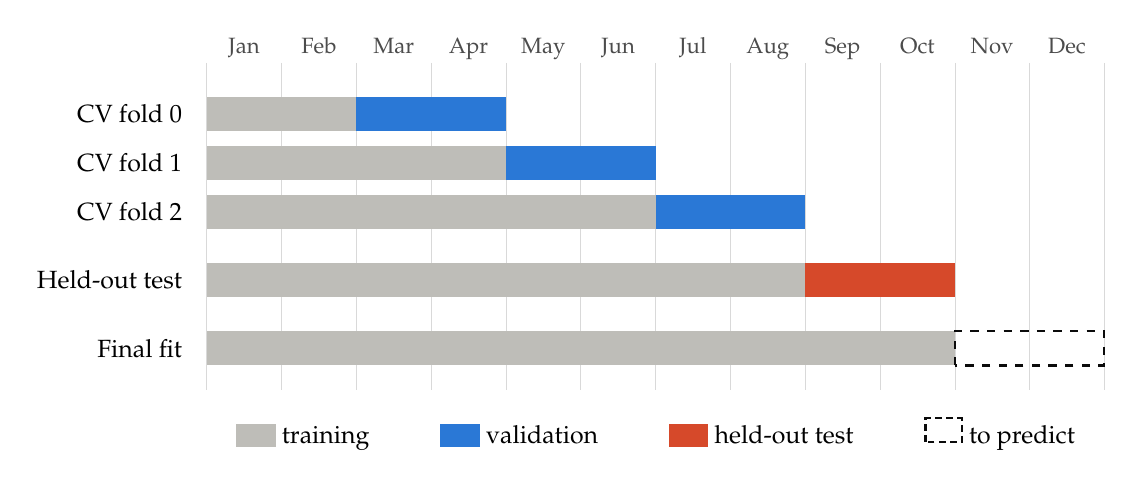
\begin{tikzpicture}[x=0.95cm,y=0.62cm,font=\small]
  \newcommand{\barrow}[4]{\fill[#4] (#2,-#1) rectangle (#3,-#1+0.7);}
  \newcommand{\swatch}[1]{\raisebox{-0.5mm}{\textcolor{#1}{\rule{0.5cm}{0.3cm}}}}
  % month grid and labels
  \foreach \ii in {0,...,12}{
    \draw[black!15,very thin] (\ii,0.4) -- (\ii,-6.3);
  }
  \foreach \mm/\ii in {Jan/0,Feb/1,Mar/2,Apr/3,May/4,Jun/5,Jul/6,Aug/7,Sep/8,Oct/9,Nov/10,Dec/11}{
    \node[anchor=base,font=\footnotesize,text=black!70] at (\ii+0.5,0.6) {\mm};
  }
  % cross-validation folds
  \barrow{1}{0}{2}{trainc}  \barrow{1}{2}{4}{valc}
  \barrow{2}{0}{4}{trainc}  \barrow{2}{4}{6}{valc}
  \barrow{3}{0}{6}{trainc}  \barrow{3}{6}{8}{valc}
  % held-out test
  \barrow{4.4}{0}{8}{trainc}  \barrow{4.4}{8}{10}{testc}
  % final fit
  \barrow{5.8}{0}{10}{trainc}
  \draw[dashed,thick,inkc] (10,-5.8) rectangle (12,-5.1);
  \node[anchor=east] at (-0.2,-0.65) {CV fold 0};
  \node[anchor=east] at (-0.2,-1.65) {CV fold 1};
  \node[anchor=east] at (-0.2,-2.65) {CV fold 2};
  \node[anchor=east] at (-0.2,-4.05) {Held-out test};
  \node[anchor=east] at (-0.2,-5.45) {Final fit};
  % legend
  \node at (6,-7.2) {\swatch{trainc}\ training\hspace{0.9cm}\swatch{valc}\ validation\hspace{0.9cm}\swatch{testc}\ held-out test\hspace{0.9cm}\tikz[baseline=-0.5mm,x=1cm,y=1cm]{\draw[dash pattern=on 2.5pt off 1.5pt,thick,inkc] (0.02,-0.03) rectangle (0.48,0.27);}\ to predict};
\end{tikzpicture}
\caption{How the 2025 data is used. The final model is fitted on all labelled months, then predicts November and December.}
\label{fig:split}
\end{figure}

\subsection{Avoiding leakage}

Everything learned from data lives inside the pipeline and is fitted on the training fold only: the median weight and the overall median of the market index. The other cleaning steps do not use other rows' information beyond what is available at prediction time. The weight is replaced by its absolute value, and a missing market index is replaced by the median of the same day computed on the features of the batch being predicted, with no price involved.

\subsection{Metric}

The main metric is the mean absolute error (MAE), in USD. RMSE and MAPE are reported for reference only. The reason is the abnormal prices described in Section~\ref{sec:outliers}: in the out-of-fold predictions of a gradient boosting model, the worst 1\% of rows (292 loads) produce 92.1\% of the total squared error but only 31.9\% of the total absolute error. RMSE therefore mostly measures a few unpredictable rows, while MAE stays readable and is expressed in dollars.

\section{What the exploration showed}

\subsection{Abnormal prices}
\label{sec:outliers}

In the development part, 533 loads (1.39\%) have a price per mile that is far from the usual range of about 1.7 to 3.0 USD: 267 are above 4 and 266 are below 1.5. I looked for a pattern and found none (Figure~\ref{fig:outliers}). The share is flat by weekday, by week of the month and by month (between about 1.2\% and 1.7\%). The number of such rows per day behaves like random counts (variance over mean of 0.92) and consecutive rows are not clustered (autocorrelation of $-0.003$). A classifier trained on all the available columns to find them is at chance level in the time-ordered folds (AUC of 0.498, 0.508 and 0.503).

\begin{figure}[htbp]
\centering
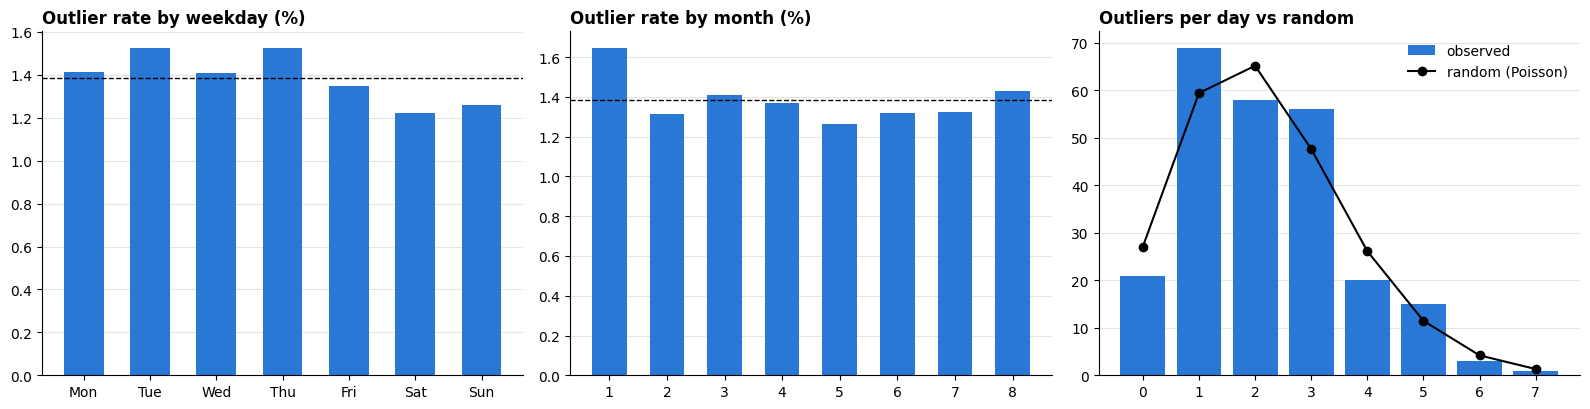
\includegraphics[width=\textwidth]{figures/outliers.png}
\caption{Share of abnormal prices by weekday and by month (dashed line is the overall 1.39\%), and number of abnormal rows per day compared with random counts.}
\label{fig:outliers}
\end{figure}

I concluded that these rows are noise in the target. They cannot be predicted from the data I have, so I kept them and chose MAE as the main metric.

\subsection{Quote signal and market index}

The two market columns behave very differently. I removed each feature in turn and measured the cross-validation MAE of three models with their default settings (Table~\ref{tab:ablation}). Removing any other feature makes the three models worse. Removing quote signal does the opposite for two of them: the error of HistGB drops from 149.1 to 132.9 USD and that of LightGBM from 151.6 to 140.3 USD. ExtraTrees is slightly worse without it (155.7 to 158.1).

\begin{table}[htbp]
\centering
\caption{Cross-validation MAE (USD) when one feature is removed. Default settings, log target.}
\label{tab:ablation}
\small
\begin{tabular}{lrrr}
\toprule
 & ExtraTrees & HistGB & LightGBM \\
\midrule
All features & 155.7 & 149.1 & 151.6 \\
Without coordinates (4 columns) & 162.5 & 154.2 & 165.3 \\
Without weight & 164.1 & 164.1 & 173.5 \\
Without market index & 163.3 & 158.5 & 164.1 \\
Without quote signal & 158.1 & 132.9 & 140.3 \\
Without equipment & 195.4 & 180.4 & 188.9 \\
Without distance & 376.9 & 447.6 & 399.5 \\
\bottomrule
\end{tabular}
\end{table}

The reason becomes clear when the relation with the rate per mile is computed month by month (Figure~\ref{fig:corr}). Quote signal has a Spearman correlation of about $+0.99$ in January to March and in June, about $-0.99$ in April, May and July, and close to zero in August. Over all the data its correlation with the price is only $-0.054$, but that is because the positive and negative months cancel each other. A model trained on these months would learn contradictory rules, and nothing in the file says which one applies in November and December. I removed quote signal.

\begin{figure}[htbp]
\centering
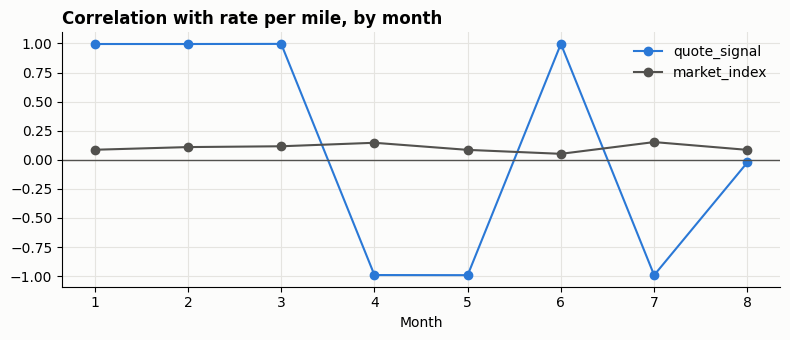
\includegraphics[width=0.78\textwidth]{figures/corr_month.png}
\caption{Spearman correlation with the rate per mile by month, on normal rows of the development part.}
\label{fig:corr}
\end{figure}

Market index is different. It is a market level that moves from day to day: the standard deviation of the daily means is 0.159, against 0.025 inside a single day, and the daily value follows the daily mean rate per mile (Spearman correlation of 0.855). Month by month its correlation with the rate per mile keeps the same sign, between 0.05 and 0.15, with a slope between 0.19 and 0.38 USD per mile for one unit of index. Removing it costs 7.6 to 12.6 USD of MAE depending on the model. The values in the validation file (0.72 to 1.10) are inside the range of the development part (0.73 to 1.47), so I kept it. It is also the only feature that depends on the date, which matters for the December chart.

\section{Models}

\subsection{Baselines and candidate models}

I compared two simple baselines (the median rate per mile multiplied by the distance, globally or by equipment), a linear regression and several tree ensembles, with raw and log-transformed targets. Table~\ref{tab:bench} shows the main ones. At this stage the models still used both market columns. Gradient boosting with a log target is clearly ahead, and CatBoost is the best of them with 132.7 USD.

\begin{table}[htbp]
\centering
\caption{Cross-validation MAE (USD) of the first models.}
\label{tab:bench}
\small
\begin{tabular}{lr}
\toprule
Model & MAE \\
\midrule
Median price (no feature) & 1,143.6 \\
Rate per mile, global & 239.2 \\
Rate per mile, by equipment & 206.7 \\
Linear regression & 157.9 \\
ExtraTrees, log target & 155.7 \\
LightGBM, log target & 151.6 \\
HistGB, log target & 149.1 \\
CatBoost, log target & 132.7 \\
\bottomrule
\end{tabular}
\end{table}

\subsection{Loss and target}

With quote signal removed, I tested two losses (squared error and absolute error, called l1) and three targets (the price, its logarithm, and the rate per mile) on the three best models. With the rate-per-mile target the model learns the price divided by the distance, and its prediction is multiplied back by the distance, so the output is a price in USD.

\begin{table}[htbp]
\centering
\caption{Cross-validation MAE (USD) by loss and target.}
\label{tab:losstarget}
\small
\begin{tabular}{lrrr}
\toprule
Loss and target & CatBoost & HistGB & LightGBM \\
\midrule
Squared, price & 128.7 & 148.2 & 160.6 \\
Squared, log & 126.4 & 132.9 & 140.3 \\
Squared, rate per mile & 121.0 & 133.9 & 151.7 \\
l1, price & 113.8 & 118.7 & 114.2 \\
l1, log & 113.6 & 117.7 & 113.2 \\
l1, rate per mile & 112.3 & 111.6 & 109.8 \\
\bottomrule
\end{tabular}
\end{table}

\begin{figure}[htbp]
\centering
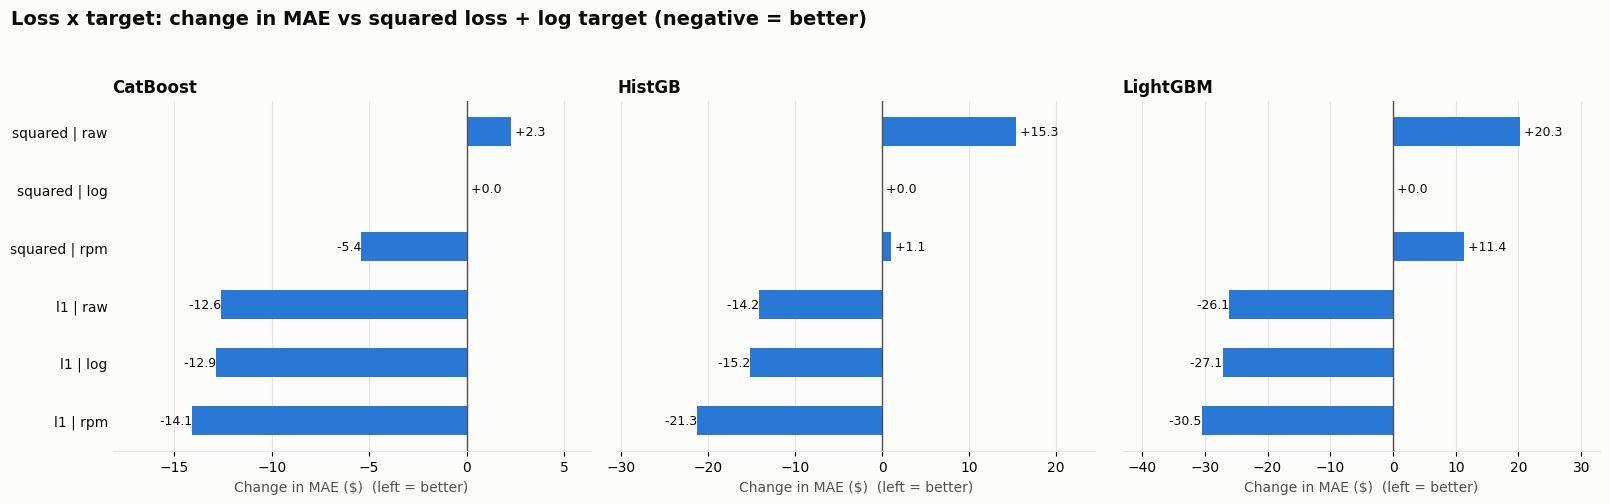
\includegraphics[width=\textwidth]{figures/loss_target.png}
\caption{Change in cross-validation MAE compared with the squared loss and log target.}
\label{fig:losstarget}
\end{figure}

The l1 loss is the real gain. It lowers the MAE by 13 to 30 USD for the three models, in all three folds each time, and it is the loss that matches the metric I care about. The rate-per-mile target is a small extra, between 1 and 6 USD compared with the log target. It is better in all three folds for HistGB and LightGBM and in two of three for CatBoost, so it is partly noise, but it is coherent with the fact that a price is roughly a rate multiplied by a distance. I kept l1 with the rate-per-mile target. The three models then sit between 110 and 112 USD.

\subsection{Hyperparameter tuning}

I tuned each model with a random search in two stages, using the same time-ordered folds and the MAE. The first stage draws 40 random configurations over wide ranges. The second stage draws 20 more inside ranges narrowed to the values used by the 8 best configurations of the first stage. A random search tries more distinct values of each parameter than a grid for the same time. The three searches took about 35 minutes in total.

\begin{table}[htbp]
\centering
\caption{Cross-validation MAE (USD) with default and tuned settings.}
\label{tab:tuning}
\small
\begin{tabular}{lrrrr}
\toprule
Model & Default & Tuned & Gain & Std over folds \\
\midrule
CatBoost & 112.34 & 107.93 & 4.42 & 3.68 \\
HistGB & 111.59 & 109.56 & 2.03 & 4.47 \\
LightGBM & 109.83 & 108.85 & 0.99 & 4.31 \\
\bottomrule
\end{tabular}
\end{table}

\begin{figure}[htbp]
\centering
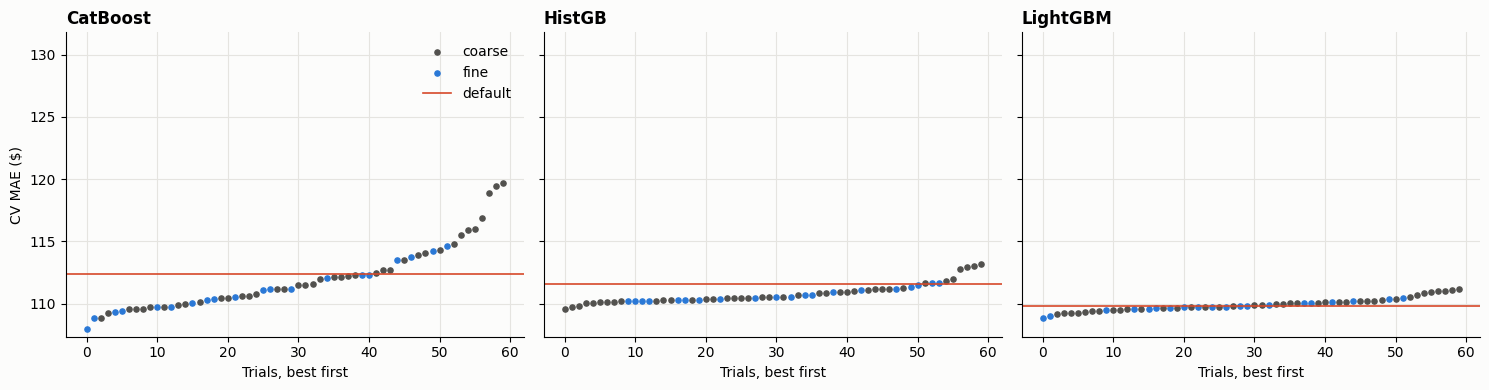
\includegraphics[width=\textwidth]{figures/tuning.png}
\caption{MAE of the 60 trials of each search, best first. The red line is the default setting.}
\label{fig:tuning}
\end{figure}

Most trials land close to the default setting, and only the worst CatBoost trials are clearly worse, so the settings matter little here (Figure~\ref{fig:tuning}). The tuned figures are also slightly optimistic, since each one is the best of 60 trials judged on the same three folds.

\subsection{Final model}

I kept CatBoost with the l1 loss and the rate-per-mile target. It has the lowest cross-validation MAE, although the three tuned models are within noise of each other (the MAE varies by about 4 USD between folds). Its settings are a depth of 4, 1,084 iterations, a learning rate of 0.052 and an L2 regularisation of 9.76. The model uses the four coordinates, the distance, the weight, the market index and the equipment, one-hot encoded into three columns, for ten input columns.

\section{Results on the held-out test}

Table~\ref{tab:test} gives the single evaluation on September and October. Every model is trained on January to August and scored on the two held-out months.

\begin{table}[htbp]
\centering
\caption{Held-out test, September and October (9,523 loads).}
\label{tab:test}
\small
\begin{tabular}{lrrrr}
\toprule
Model & MAE & RMSE & MAPE (\%) & Median error (\%) \\
\midrule
Baseline, rate per mile by equipment & 229.10 & 670.66 & 10.49 & 6.80 \\
CatBoost, squared loss, log target & 162.49 & 650.08 & 6.88 & 4.31 \\
CatBoost, l1 loss, rate per mile & 164.58 & 649.82 & 6.95 & 4.44 \\
CatBoost tuned (final) & 164.58 & 649.77 & 6.94 & 4.44 \\
\bottomrule
\end{tabular}
\end{table}

The final model reaches an MAE of 164.6 USD, against 229.1 USD for the best simple baseline. The error is 172.0 USD in September and 157.5 USD in October. Two things need a comment.

First, the test error is much higher than the cross-validation error of 107.9 USD. Second, the gains brought by the l1 loss, the rate-per-mile target and the tuning in cross-validation are not visible here: the three CatBoost versions are between 162.5 and 164.6 USD, a difference that is small compared with the 4 USD variation between folds.

\subsection{Why the test error is higher}

The error is mostly one-sided. On normal rows (rate per mile between 1.5 and 4), the model underestimates the price in every fold, but much more on the test (Table~\ref{tab:bias} and Figure~\ref{fig:shift}).

\begin{table}[htbp]
\centering
\caption{Mean error and MAE of the final model on normal rows. A positive error means the model underestimates.}
\label{tab:bias}
\small
\begin{tabular}{lrrr}
\toprule
 & Mean error (USD) & Mean error (USD per mile) & MAE (USD) \\
\midrule
CV fold 0 & 56.99 & 0.051 & 65.09 \\
CV fold 1 & 48.03 & 0.046 & 59.84 \\
CV fold 2 & 41.60 & 0.038 & 52.36 \\
Test, Sep to Oct & 109.13 & 0.101 & 109.52 \\
\bottomrule
\end{tabular}
\end{table}

\begin{figure}[htbp]
\centering
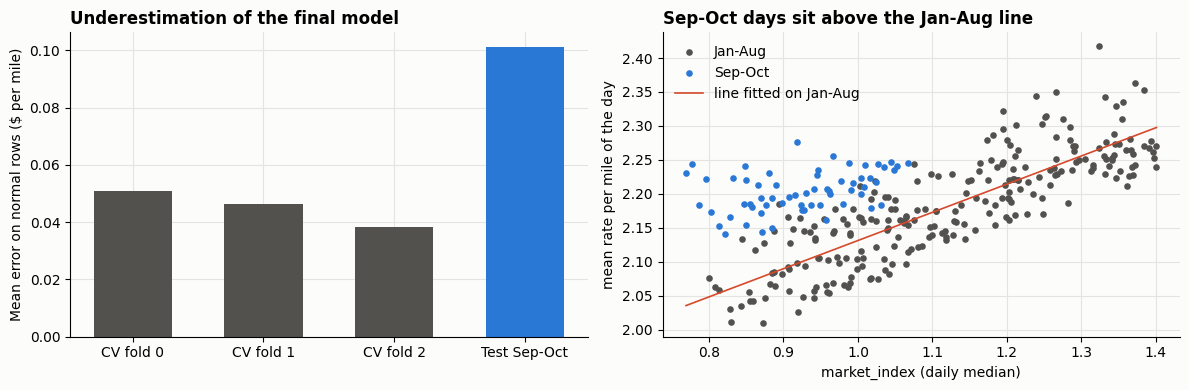
\includegraphics[width=\textwidth]{figures/level_shift.png}
\caption{Left: mean underestimation on normal rows. Right: one point per day, with the market index on the horizontal axis and the mean rate per mile on the vertical axis. The line is fitted on January to August.}
\label{fig:shift}
\end{figure}

The right panel shows the cause. From January to August, days with a higher market index have a higher rate per mile, and the points follow a line. In September and October the market index is in the lower part of its range (the blue points lie between about 0.77 and 1.1), but the days sit above the line by 0.10 USD per mile on average. The model learned that a low index means a lower price, and that stopped being true in these two months. The shift is visible in the data itself, before any model is involved.

So the cross-validation figure is optimistic for a period that comes after the training data, and the test figure of 164.6 USD is the one I report. After seeing the test result I looked at the test labels to understand the gap. I made no change to the model, the features or the settings because of it.

The final model is trained again on all labelled months, January to October, so it has seen the September and October level. That should help with the shift, but I cannot measure it, because there are no labels for November and December, and the level may move again.

\section{Predictions and December chart}
\label{sec:december}

\subsection{Validation file}

The completed file \texttt{validation\_predictions.csv} has the 12,000 rows with the columns \texttt{load\_id} and \texttt{predicted\_rate}, all positive, and it passes the check of \texttt{score.py}. The predictions go from 186.8 to 6,706.9 USD with a median of 1,995.0 USD. As a sanity check, I compared the predicted rate per mile with the labelled one. The 1\%, 50\% and 99\% quantiles are 1.72, 2.10 and 2.93 for the predictions, against 1.67, 2.15 and 3.18 in the labelled data. The predicted means by equipment are a little lower than the labelled ones (Dry Van 2.05 against 2.12, Flatbed 2.21 against 2.29, Reefer 2.31 against 2.38), which goes in the same direction as the underestimation seen on the test.

\subsection{Fixed December route}

The December file only contains the route, the distance, the equipment, the weight and the date, while the model also needs the coordinates and the market index. I completed these two. The coordinates are those of the same route in the labelled data. The market index of each day is the median of that day in the validation file, which has loads on every day of December. The original file is not modified, and the completed copy is saved as \texttt{december\_predictions.csv}. The scorer validated the 31 predictions and produced Figure~\ref{fig:december}.

\begin{figure}[htbp]
\centering
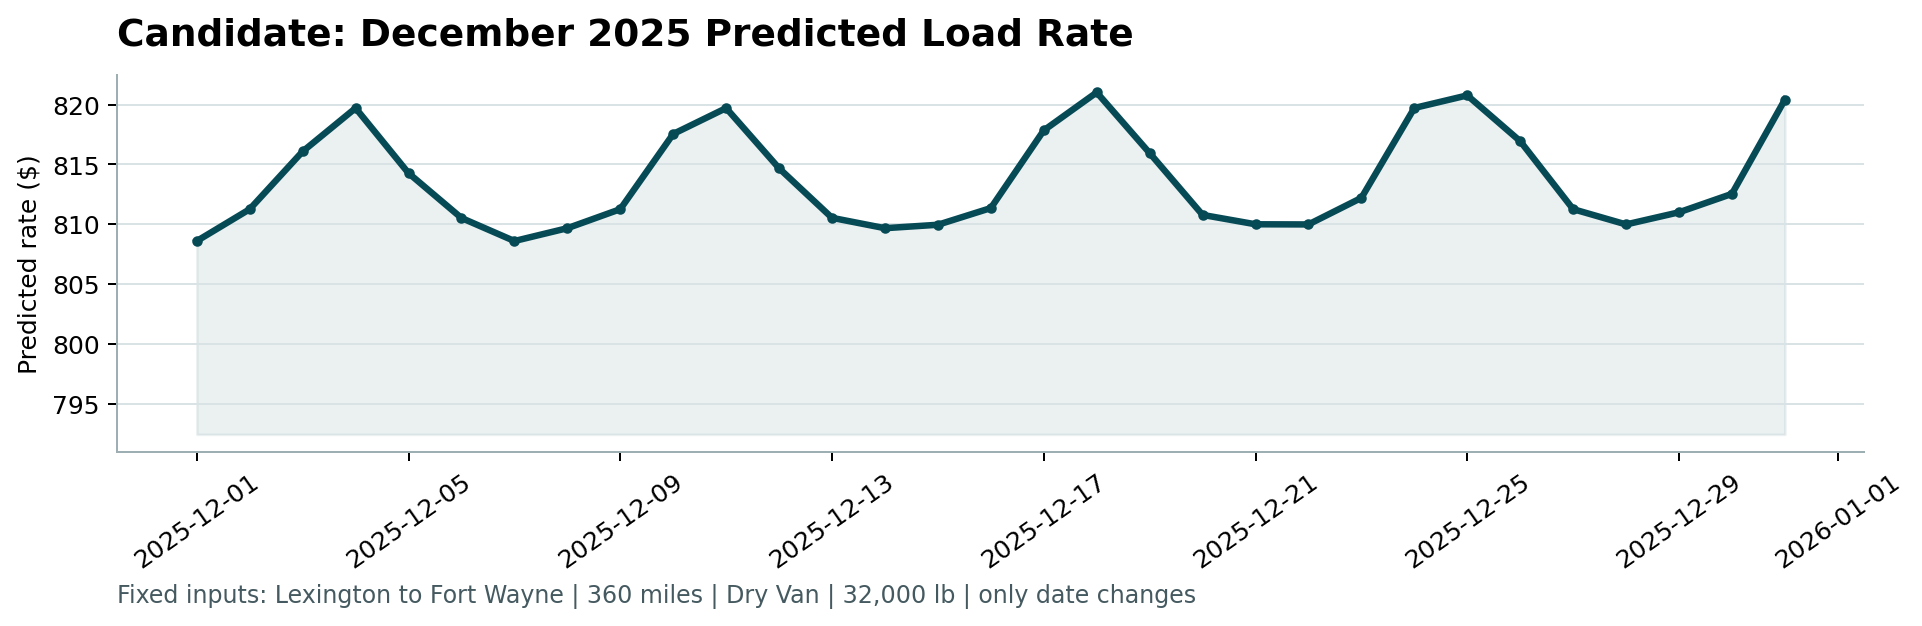
\includegraphics[width=0.9\textwidth]{figures/candidate_december.png}
\caption{Fixed December prediction chart produced by \texttt{score.py}: Lexington to Fort Wayne, 360 miles, Dry Van, 32,000 lb.}
\label{fig:december}
\end{figure}

The predicted rate goes from 808.6 to 821.0 USD over the month, a spread of about 1.5\%. The vertical axis of the chart is zoomed, so the swings look larger than they are. The curve repeats a cycle of seven days. In the first week, for example, the market index rises from 0.833 on Monday to 1.025 on Thursday and falls to 0.829 on Sunday, and the prediction goes from 808.6 to 819.7 USD and back to 808.6 USD. The route is fixed and the date is not a feature of the model, so the market index is the only input that changes from one day to the next. The chart is therefore the response of the model to the daily market index. Its level carries the same uncertainty as the test result above.

\section{Using the model}

{\sloppy
To make the model usable outside the notebook, the final pipeline is saved in \texttt{freight\_rate\_model.joblib}, and a small Streamlit application, \texttt{app.py}, loads it. The application has two modes. In the first, one chooses the cities, the distance, the weight, the equipment, the date and the market index, and it returns the predicted rate and the rate per mile. The coordinates are read from the training data, so only the 64 cities of the training data are offered. In the second mode, one uploads a file with the nine columns the model needs (four coordinates, distance, weight, market index, equipment and date), and the predictions can be downloaded. The validation file works as it is. Figure~\ref{fig:app} shows the first mode. The commands to run the notebook and the application are in the \texttt{README.md} of the repository. The seeds are fixed, so running the notebook again gives the same results.\par}

\begin{figure}[H]
\centering
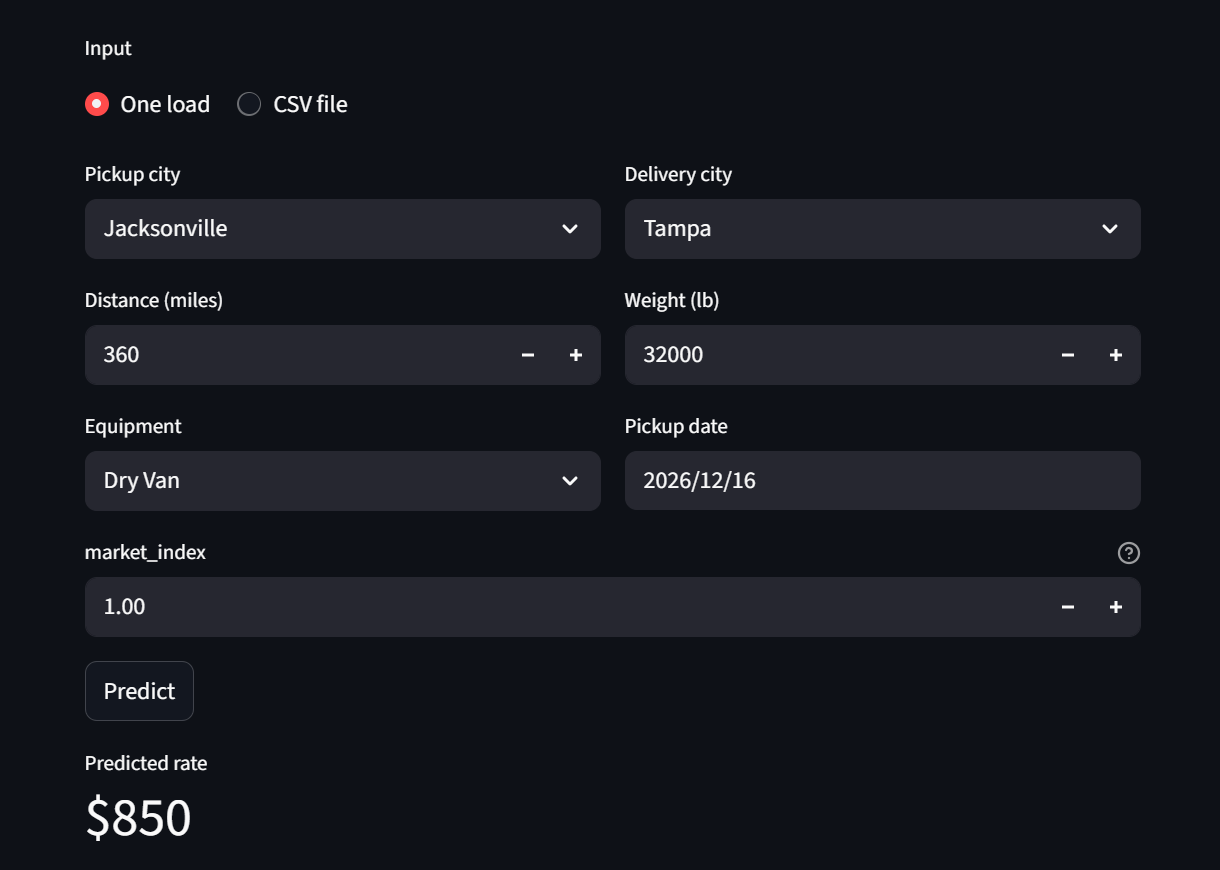
\includegraphics[width=0.8\textwidth]{figures/app_screenshot.png}
\caption{The application in its single-load mode.}
\label{fig:app}
\end{figure}

\section{Limits}

The main limit is the shift of the price level seen in September and October. I cannot say how the level behaves in November and December, so the December chart is best read for its shape.

With ten months of data, no yearly pattern can be learned, so I did not use calendar features such as the month.

The abnormal prices, about 1.4\% of the loads, cannot be predicted from the columns provided. They are present in the test as well and they raise every error figure.

Quote signal changes meaning from month to month, so I left it out. If the regime of a given month were known, it could carry information.

A variable holding the recent level of prices would be the natural way to follow a shift like the one of September and October. The validation file contains no prices, so I could not build one here.

\end{document}
